%%% Version 2.1 Generated 2013/10/17 %%%
%%% You will need to have the following packages installed: datetime, fmtcount, etoolbox, fcprefix, which are normally inlcuded in WinEdt. %%%
%%% In http://www.ctan.org/ you can find the packages and how to install them, if necessary. %%%

%\documentclass{frontiersENG} % for Engineering articles
%\documentclass{frontiersSCNS} % for Science articles
\documentclass{frontiersMED} % for Medicine articles

\usepackage{url,lineno,listings}
\linenumbers

\lstset{ %
language=C++,                % choose the language of the code
basicstyle=\footnotesize,       % the size of the fonts that are used for the code
numbers=right,                   % where to put the line-numbers
numberstyle=\footnotesize,      % the size of the fonts that are used for the line-numbers
stepnumber=1,                   % the step between two line-numbers. If it is 1 each line will be numbered
numbersep=5pt,                  % how far the line-numbers are from the code
backgroundcolor=\color{white},  % choose the background color. You must add \usepackage{color}
showspaces=false,               % show spaces adding particular underscores
showstringspaces=false,         % underline spaces within strings
showtabs=false,                 % show tabs within strings adding particular underscores
frame=single,           % adds a frame around the code
tabsize=2,          % sets default tabsize to 2 spaces
captionpos=b,           % sets the caption-position to bottom
breaklines=true,        % sets automatic line breaking
breakatwhitespace=false,    % sets if automatic breaks should only happen at whitespace
escapeinside={\%*}{*)}          % if you want to add a comment within your code
}


% Leave a blank line between paragraphs in stead of using \\

\copyrightyear{}
\pubyear{}

\def\journal{Neuroinformatics}%%% write here for which journal %%%
\def\DOI{}
\def\articleType{Methods}
\def\keyFont{\fontsize{8}{11}\helveticabold }
\def\firstAuthorLast{Lowekamp {et~al.}} %use et al only if is more than 1 author
\def\Authors{Bradley Lowekamp\,$^{1,*}$, David T. Chen\,$^{1}$, Luis Ibanes\,$^2$ and Danial Blezek\,$^3$}
% Affiliations should be keyed to the author's name with superscript numbers and be listed as follows: Laboratory, Institute, Department, Organization, City, State abbreviation (USA, Canada, Australia), and Country (without detailed address information such as city zip codes or street names).
% If one of the authors has a change of address, list the new address below the correspondence details using a superscript symbol and use the same symbol to indicate the author in the author list.
\def\Address{$^{1}$Office of High Performance and Communication, National Library of Medicine, Bethesda, MD, USA \\
$^{2}$Kitware, Clifton Park, NY, USA \\
$^{3}$Mayo Graduate School of Medicine, Biomedical Engineering Department, Rochester, MN, USA}
% The Corresponding Author should be marked with an asterisk
% Provide the exact contact address (this time including street name and city zip code) and email of the corresponding author
\def\corrAuthor{Bradley Lowekamp}
\def\corrAddress{Office of High Performance and Communication, National Library of Medicine, 8600 Rockville Pike, Bethesda, 20894, MD, USA}
\def\corrEmail{blowekamp@mail.nih.gov}

% \color{FrontiersColor} Is the color used in the Journal name, in the title, and the names of the sections.


\begin{document}
\onecolumn
\firstpage{1}

\title[The Design of SimpleITK]{The Design of SimpleITK}
\author[\firstAuthorLast ]{\Authors}
\address{}
\correspondance{}
\extraAuth{}% If there are more than 1 corresponding author, comment this line and uncomment the next one.
\topic{}% If your article is part of a Research Topic, please indicate here which.

\maketitle

\begin{abstract}

%%% Leave the Abstract empty if your article falls under any of the following categories: Editorial Book Review, Commentary, Field Grand Challenge, Opinion or specialty Grand Challenge.
\section{}
SimpleITK is a new interface to the Insight Segmentation and Registration Toolkit (ITK) designed to facilitate rapid prototyping and educational activities, through access via additional programming languages. ITK is a templated C++ library of image processing algorithms and frameworks for biomedical and other applications, and it was designed to be generic, flexible and extensible. Initially, ITK provided a direct wrapping interface to languages such as Python and Tcl through the WrapITK system. Unlike WrapITK, which exposed ITK’s complex templated interface, SimpleITK was designed to provide an easy to use and simplified interface to ITK's algorithms. It includes procedural methods, hides ITK's demand driven pipeline, and provides a template-less layer.   Also SimpleITK provides practical conveniences such as binary distribution packages and overloaded operators. Our user-friendly design goals dictated a departure from the direct interface wrapping approach WrapITK has taken, towards a new façade class structure that only exposes the required functionality, hiding ITK’s extensive template use. Internally SimpleITK utilizes a manual description of each filter with code-generation and advanced C++ meta-programming to provide the higher-level interface, bringing the capabilities of ITK to a larger audience.

\tiny
%All article types: you may provide up to 8 keywords; at least 5 are mandatory.
 \keyFont{ \section{Keywords:}  Software Design, Insight Toolkit segmentation, Image Processing, Computer-Assisted, interactive }
\end{abstract}

\section{Introduction}
The proper practice of the scientific method requires the systematic
verification of reproducibility of published reports
\cite{Popper1934}. Ideally, this verification must be performed by
independent observers in order for it to be trustable \cite{Popper1963}. In
the context of computational science, the reports of scientific
research, must include the means and the complete details required to
enable independent groups to fully replicate the results that are
being published. In particular, they should include: data, reports,
list of experimental parameters, and software.

Open source software provides public implementations of state of the
art algorithms, that facilitate the accelerated advancement of a
field, through a more efficient research lifecycle, and through more
practical education. The National Library of Medicine’s Insight
Segmentation and Registration Toolkit (ITK) is a leading open source
software for biomedical image analysis. Since 1999, it has been used
in fields as varied as brain registration for neuroscience, microscopy
image analysis, radiation treatment planning, image segmentation for
brain tumors, and processing of electron microscopy, as well as
non-medical applications such as satellite imagery and industrial
inspection.

Our fundamental goal in developing SimpleITK was to grow the user base
of ITK.  Whereas direct use of the ITK programming interface requires
expertise in templated C++, SimpleITK was designed to be accessible
from a variety of languages.  Furthermore SimpleITK has a
straightforward interface that does not require knowledge of the
intricacies of ITK’s templated types. By lowering the bar to access
ITK’s portfolio of image processing algorithms we hope to further the
goals of open source and open science.

\subsection{The Insight Segmentation and Registration Toolkit}

The Insight Segmentation and Registration Toolkit (ITK) was originally
conceived as public software tools for the analysis of the Visible
Human Project by the National Library of Medicine (NLM) with
partnership from six other institutes at the National Institutes of
Health (NIH). During the initial development the mission of ITK was
outlined as: “a software foundation for future research, an archival
repository of image processing algorithms, a catalog of validation
techniques, as well as a platform for advanced product development”
\cite{Yoo2002}. NLM has continued to support ITK through Algorithm Adaptors
and Data Distribution (A2D2) programs and on going maintenance, while
trying to foster the development of a sustainable open source
community. In 2010 NLM initiated a major revision and refactoring of
the toolkit funded by the American Recovery and Reinvestment
Act. Among the objectives outlined is to simplify ITK.

Through the contributions of the ITK community and continued funding
the scope of ITK has continued to grow. The version 4 refactoring
separated ITK into a modular structure which now contains over 100
modules. The segmentation algorithms available in ITK include region
growing, level sets, markov random field classifiers, watersheds and
other statistical classifiers. The registration framework is designed
to be modular with the distinct parts for a transform, interpolator,
transform, optimizer, and image similarity metric along with support
for multi-resolution methods. ITK also contains data-structures for
spatial object, histograms, finite element meshes, quad-edge meshes,
neural networks, images and narrow band level-sets. There are a large
number of third party libraries that are supported and used for input
and output. Additionally there are a numerous image filters algorithms
available including mathematical morphology, smoothing, deconvolution,
distance maps, fast marching, image fusion, image statistics,
geometric filters, and image sources among many others. ITK contains a
wealth of algorithms, interfaces and data-structures to provide a
platform for research in algorithm development and a collection of
image processing algorithms.

The design of ITK focuses on providing a powerful and flexible
platform to allow for research, experimentation and development of
algorithms. To that end one of the notable implementation details in
ITK is the extensive use of C++ templates. The ITK image class is a
templated structure over both the pixel type as well as the image
dimension. The choice pervades all areas of the toolkit. Image filters
must be templated over the image type. Also the structures and objects
used with the image classes are also templated. These data structures
include image iterators, points, and indices. The results of this
interface design can be seen the code listing, from the ITK Software
Guide \cite{Ibanez2003}.

\lstinputlisting[firstline=36, lastline=74]{itkGaussianExample.cxx}

Notably missing from the design goals of ITK are usability and accessibility.





%\begin{methods}
\section{Material \& Methods}

Text Text Text Text Text Text  Text Text Text Text Text Text Text Text Text  Text Text Text Text Text Text Text Text Text Text  Text Text Text Text Text Text  Text Text.  \cite{Neuro2013} might want to know about  text text text text Text Text Text Text  Text Text Text Text Text Text  Text Text. \citep{Gene2012} might want to know about  text text text text
Text Text Text Text Text Text  Text Text Text Text Text Text Text Text Text  Text Text Text Text Text Text Text Text Text Text  Text Text Text Text Text Text  Text Text.  \cite{Neurobot2013} might want to know about  text text text text

\begin{table}[!t]
\processtable{Maximum size of the Manuscript\label{Tab:01}}
{\begin{tabular}{lllll}\toprule
 & Abstract max. legth (incl. spaces) & Figures or tables & Manuscript max. length & Final PDF length\\\midrule
Clinical Case Study & & & &\\
Clinical Trial & & & &\\
Hypothesis and Theory & & & &\\
Methods & 2000 characters  & 15 & 12000 words & 12 pages\\
Original Research & & & &\\
Review & & & &\\
Technology Report & & & &\\
Focused Review & 2000 characters & 5 & 5000 words & 5 pages\\
CPC &  1250 characters& 6 & 2500 words & 4 pages\\
Perspective & 1250 characters & 2 & 3000 words & 3 pages\\
Mini Review & & & &\\
Classification & 1250 characters & 10 & 2000 words & 12 pages\\
Editorial & none & none & 1000 words & 1 page \\
Book review & & & &\\
Frontiers Commentary & none & 1 & 1000 words & 1 page\\
General Commentary & & & &\\
Field Grand Challenge & & & &\\
Opinion & none & 1 & 2000 words & 2 pages\\
Specialty Grand Challenge& & & &\\\botrule
\end{tabular}}{}
\end{table}

Please note that very large tables (covering several pages) cannot be included in the final PDF for reasons of space. These tables will be published as supplementary material on the online article abstract page at the time of acceptance. The author will notified during the typesetting of the final article if this is the case. A link in the final PDF will direct to the online material.

\subsection{Original Research Articles, Clinical Trial Articles, and Technology Reports}

For Original Research Articles, Clinical Trial Articles, and Technology Reports the section headings should be those appropriate for your field and the research itself. It is recommended to organize your manuscript in the following sections or their equivalents for your field:

\begin{itemize}
%for bulleted list, use itemize
\item Introduction: Succinct, with no subheadings.
\item Materials and Methods: This section may be divided by subheadings. This section should contain sufficient detail so that when read in conjunction with cited references, all procedures can be repeated.
\item Results: This section may be divided by subheadings. Footnotes should not be used and have to be transferred into the main text.
\item Discussion: This section may be divided by subheadings. Discussions should cover the key findings of the study: discuss any prior art related to the subject so to place the novelty of the discovery in the appropriate context; discuss the potential short-comings and limitations on their interpretations; discuss their integration into the current understanding of the problem and how this advances the current views; speculate on the future direction of the research and freely postulate theories that could be tested in the future.
\end{itemize}

Please note that the Material and Methods section can be placed in any of the following ways: before Results, before Discussion or after Discussion.

\subsection{Clinical Case Studies}

For Clinical Case Studies the following sections are mandatory:

\begin{itemize}
%for bulleted list, use itemize
\item Introduction: Include symptoms at presentation, physical exams and lab results.
\item Background: This section may be divided by subheadings. Include history and review of similar cases.
\item Results: This section may be divided by subheadings. Include diagnosis and treatment.
\item Concluding Remarks
\end{itemize}

%\end{methods}



\section{Results}

Frontiers requires figures to be submitted individually, in the same order as they are referred to in the manuscript. Figures will then be automatically embedded at the bottom of the submitted manuscript. Kindly ensure that each table and figure is mentioned in the text and in numerical order. Permission must be obtained for use of copyrighted material from other sources (including the web). Please note that it is compulsory to follow figure instructions. Figures which are not according to the guidelines will cause substantial delay during the production process.

\begin{table}[!t]
\processtable{Resolution Requirements for the figures\label{Tab:02}}
{\begin{tabular}{lllll}\toprule
Image Type & Description & Format & Color Mode & Resolution\\\midrule
Line Art & An image composed of lines and text,  & TIFF, JPEG & RGB, Bitmap & 900 - 1200 dpi\\
           & which does not contain tonal or shaded areas.& & &\\
           Halftone & A continuous tone photograph, which contains no text. & TIFF, EPS, JPEG & RGB, Grayscale & 300 dpi\\
Combination & Image contains halftone + text or line art elements. & TIFF, JPEG & RGB,Grayscale & 600 - 900 dpi\\\botrule
\end{tabular}}{This is a footnote}
\end{table}

\begin{equation}
\sum x+ y =Z\label{eq:01}
\end{equation}

\textbf{Table\ref{Tab:02}} shows the resolution requirements for the figures. The figures must be legible:
\begin{enumerate}
\item The smallest visible text is no less than 8 points in height, when viewed at actual size.
\item Solid lines are not broken up.
\item Image areas are not pixelated or stair stepped.
\item Text is legible and of high quality.
\item Any lines in the graphic are no smaller than 2 points width.
\item The actual size of the figure must be of at least 8.5 cm.
\end{enumerate}

\section{Discussion}

Text Text Text Text Text Text  Text Text Text Text Text Text Text Text Text  Text Text Text Text Text Text Text Text Text Text.
Additional Requirements:
\subsection{Corrections}

Minor corrections to published articles can be communicated to the Frontiers Production Office at production.office@frontiersin.org. If you need to communicate important changes to an article please submit a General Commentary. Submit the article with the title “Erratum: Original Title of Article”.

\subsection{Commentaries on Articles}

At the beginning of your manuscript provide the citation of the article commented on.

\subsection{Focused Reviews}

For Tier 2 invited Focused Reviews the sections Introduction, Material and Methods, Results, and Discussion are recommended. In addition the authors must submit a short biography of the corresponding author(s). This short biography has a maximum of 600 characters, including spaces.

A picture (5 x 5 cm, in *.tif or *.jpg, min 300 dpi) must be submitted along with the biography in the manuscript and separately during figure upload.
Focused Reviews highlight and explain key concepts of your work. Please highlight a minimum of four and a maximum of ten key concepts in bold in your manuscript and provide the definitions/explanations at the end of your manuscript under “Key Concepts”. Each definition has a maximum of 400 characters, including spaces.

\subsection{Human Search and Animal Research}

All experiments on live vertebrates or higher invertebrates must be performed in accordance with relevant institutional and national guidelines and regulations. In the manuscript, authors must identify the committee approving the experiments and must confirm that all experiments conform to the relevant regulatory standards. For manuscripts reporting experiments on human subjects, authors must identify the committee approving the experiments and must also include a statement confirming that informed consent was obtained from all subjects. In Original Research Articles and Clinical Trial Articles these statements should appear in the Materials and Methods section.

\subsection{Clinical Trial Registration}

Clinical trials should be registered in a public trials registry in order to become the object of a publication at Frontiers. Trials must be registered at or before the start of patient enrollment. A clinical trial is defined as"any research study that prospectively assigns human participants or groups of humans to one or more health-related interventions to evaluate the effects on health outcomes."(\url{www.who.int/ictrp/en}). A list of acceptable registries can be found at \url{www.who.int/ictrp/en and www.icmje.org}.

\subsection{Inclusion of Proteomics Data}

Authors should provide relevant information relating to how the peptide/protein matches were undertaken, including methods used to process and analyze data, false discovery rates (FDR) for large-scale studies and threshold or cut-off rates for peptide and protein matches. Further information could include software used, mass spectrometer type, sequence database and version, number of sequences in database, processing methods, mass tolerances used for matching, variable/fixed modifications, allowable missed cleavages, etc.

Authors should provide as supplementary material information used to identify proteins and/or peptides. This should include information such as accession numbers, observed mass (m/z), charge, delta mass, matched mass, peptide/protein scores, peptide modification, miscleavages, peptide sequence, match rank, matched species (for cross species matching), number of peptide matches, ambiguous protein/peptide matches should be indicated, etc.
For quantitative proteomics analyses authors should provide information to justify the statistical significance including biological replicates, statistical methods, estimates of uncertainty and the methods used for calculating error.

For peptide matches with biologically relevant post-translational modifications (PTM) and for any protein match that has occurred using a single mass spectrum, authors should include this information as raw data, annotated spectra or submit data to an online repository (recommended option).
Authors are encouraged to submit raw or matched data and 2-DE images to public proteomics repositories. Submission codes and/or links to data should be provided within the manuscript.

\subsection{Data Sharing}

Frontiers supports the policy of data sharing, and authors are advised to make freely available any materials and information described in their article, and any data relevant to the article (while not compromising confidentiality in the context of human-subject research) that may be reasonably requested by others for the purpose of academic and non-commercial research. In regards to deposition of data and data sharing through databases, Frontiers urges authors to comply with the current best practices within their discipline.

\section*{Disclosure/Conflict-of-Interest Statement}
%All relationships financial, commercial or otherwise that might be perceived by the academic community as representing a potential conflict of interest must be described. If no such relationship exists, authors will be asked to declare that the research was conducted in the absence of any commercial or financial relationships that could be construed as a potential conflict of interest.
The authors declare that the research was conducted in the absence of any commercial or financial relationships that could be construed as a potential conflict of interest.

\section*{Acknowledgement}
Text Text Text Text Text Text  Text Text Text Text Text Text Text Text  Text Text Text Text Text Text Text Text Text  Text Text Text.

\paragraph{Funding\textcolon} Text Text Text Text Text Text  Text Text.

\section*{Supplemental Data}
Text Text Text Text Text Text  Text Text Text Text Text Text Text Text Text  Text Text Text Text Text Text Text Text Text  Text Text Text.

%\bibliographystyle{frontiersinSCNS&ENG} % for Science and Engineering articles
\bibliographystyle{frontiersinMED} % for Medicine articles
\bibliography{test}

\section*{Figures}

%%% Use this if adding the figures directly in the mansucript, if so, please remember to also upload the files when submitting your article
%%% There is no need for adding the file termination, as long as you indicate where the file is saved. In the examples below the files (logo1.jpg and logo2.eps) are in the Frontiers LaTeX folder
%%% If using *.tif files convert them to .jpg or .png

%\begin{figure}
%\begin{center}
%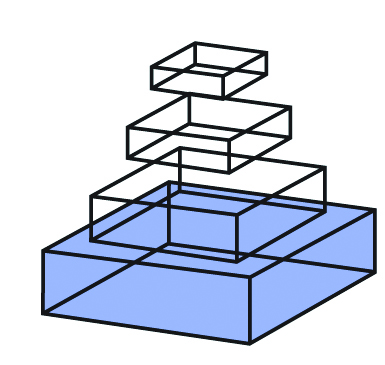
\includegraphics[width=3.5cm]{logo1}% This is a *.jpg file
%\end{center}
% \textbf{\refstepcounter{figure}\label{fig:01} Figure \arabic{figure}.}{ Enter the caption for your figure here.  Repeat as  necessary for each of your figures }
%\end{figure}

%\begin{figure}
%\begin{center}
%
\includegraphics[width=3.5cm]{logo2}% This is an *.eps file
%\end{center}
% \textbf{\refstepcounter{figure}\label{fig:02} Figure \arabic{figure}.}{ Enter the caption for your figure here.  Repeat as  necessary for each of your figures }
%\end{figure}

 \textbf{Figure 1.}{ Enter the caption for your figure here.  Repeat as  necessary for each of your figures.}\label{fig:01}% If you don't add the figures in the LaTeX files, please upload them when submitting the article.

%%% Frontiers will add the figures at the end of the provisional pdf automatically %%%

%%% The use of LaTeX coding to draw Diagrams/Figures/Structures should be avoided. They should be external callouts including graphics.

\end{document}
